\documentclass[sigconf]{acmart}

\usepackage{calc}
\usepackage{amsmath}
\usepackage{mathtools}
\usepackage{textcomp}
\usepackage{amssymb}
\usepackage{tikz}

\makeatletter
\newcommand*{\da@rightarrow}{\mathchar"0\hexnumber@\symAMSa 4B }
\newcommand*{\da@leftarrow}{\mathchar"0\hexnumber@\symAMSa 4C }
\newcommand*{\xdashrightarrow}[2][]{%
  \mathrel{%
    \mathpalette{\da@xarrow{#1}{#2}{}\da@rightarrow{\,}{}}{}%
  }%
}
\newcommand{\xdashleftarrow}[2][]{%
  \mathrel{%
    \mathpalette{\da@xarrow{#1}{#2}\da@leftarrow{}{}{\,}}{}%
  }%
}
\newcommand*{\da@xarrow}[7]{%
  % #1: below
  % #2: above
  % #3: arrow left
  % #4: arrow right
  % #5: space left
  % #6: space right
  % #7: math style
  \sbox0{$\ifx#7\scriptstyle\scriptscriptstyle\else\scriptstyle\fi#5#1#6\m@th$}%
  \sbox2{$\ifx#7\scriptstyle\scriptscriptstyle\else\scriptstyle\fi#5#2#6\m@th$}%
  \sbox4{$#7\dabar@\m@th$}%
  \dimen@=\wd0 %
  \ifdim\wd2 >\dimen@
    \dimen@=\wd2 %
  \fi
  \count@=2 %
  \def\da@bars{\dabar@\dabar@}%
  \@whiledim\count@\wd4<\dimen@\do{%
    \advance\count@\@ne
    \expandafter\def\expandafter\da@bars\expandafter{%
      \da@bars
      \dabar@
    }%
  }%
  \mathrel{#3}%
  \mathrel{%
    \mathop{\da@bars}\limits
    \ifx\\#1\\%
    \else
      _{\copy0}%
    \fi
    \ifx\\#2\\%
    \else
      ^{\copy2}%
    \fi
  }%
  \mathrel{#4}%
}
\makeatother

\copyrightyear{2019}
\acmYear{2019}
\setcopyright{acmcopyright}
\acmConference[CEE-SECR'19]{Central and Eastern European Software Engineering Conference Russia}{November 14--15(16), 2019}{St.Petersburg, Russia}
%\acmBooktitle{2nd Joint International Workshop on Graph Data Management
%Experiences \& Systems (GRADES) and Network Data Analytics (NDA)
%(GRADES-NDA'19), June 30-July 5, 2019, Amsterdam, Netherlands}
%\acmPrice{15.00}
%\acmDOI{10.1145/3327964.3328503}
%\acmISBN{978-1-4503-6789-9/19/06}

\begin{document}

\title[IDEs-Friendly Interprocedural Analyser]{IDEs-Friendly Interprocedural Analyser}

\author{Ilya Nozhkin}
\affiliation{
  \institution{Saint Petersburg State University}
  \streetaddress{7/9 Universitetskaya nab.}
  \city{St. Petersburg}
  \country{Russia}
  \postcode{199034}
}
\email{nozhkin.ii@gmail.com}

\author{Semyon Grigorev}
\orcid{0000-0002-7966-0698}
\affiliation{
  \institution{Saint Petersburg State University}
  \streetaddress{7/9 Universitetskaya nab.}
  \city{St. Petersburg}
  \country{Russia}
  \postcode{199034}
}
\affiliation{
  \institution{JetBrains Research}
  \streetaddress{Universitetskaya nab., 7-9-11/5A}
  \city{St. Petersburg}
  \country{Russia}
  \postcode{199034}
}
\email{s.v.grigoriev@spbu.ru}
\email{semen.grigorev@jetbrains.com}


\begin{abstract}
We propose an extensible framework for interprocedural static code analysis implementation.
Our solution is based on CFL-reachability: analysis is formulated in terms of context-free constrained reachability in the interprocedural graph.
Extensible architecture allows one to implement new analysis and integrate it into the IDE of choice or static code analysis tool.
To demonstrate the abilities of our solution, we implement the plugin which provides basic taint analysis and variable flow analysis upon ReSharper infrastructure.
We demonstrate its applicability for real-world problems.
\end{abstract}


\begin{CCSXML}
<ccs2012>
<concept>
<concept_id>10011007.10010940.10010992.10010998.10011000</concept_id>
<concept_desc>Software and its engineering~Automated static analysis</concept_desc>
<concept_significance>500</concept_significance>
</concept>
<concept>
<concept_id>10011007.10011006.10011066.10011069</concept_id>
<concept_desc>Software and its engineering~Integrated and visual development environments</concept_desc>
<concept_significance>500</concept_significance>
</concept>
<concept>
<concept_id>10011007.10011074.10011099.10011102</concept_id>
<concept_desc>Software and its engineering~Software defect analysis</concept_desc>
<concept_significance>500</concept_significance>
</concept>
<concept>
<concept_id>10011007.10010940.10011003.10011114</concept_id>
<concept_desc>Software and its engineering~Software safety</concept_desc>
<concept_significance>300</concept_significance>
</concept>
<concept>
<concept_id>10003752.10003766.10003771</concept_id>
<concept_desc>Theory of computation~Grammars and context-free languages</concept_desc>
<concept_significance>300</concept_significance>
</concept>
</ccs2012>
\end{CCSXML}

\ccsdesc[500]{Software and its engineering~Automated static analysis}
\ccsdesc[500]{Software and its engineering~Integrated and visual development environments}
\ccsdesc[500]{Software and its engineering~Software defect analysis}
\ccsdesc[300]{Software and its engineering~Software safety}
\ccsdesc[300]{Theory of computation~Grammars and context-free languages}

\keywords{Static code analysis, interprocedural analysis, CFL-reachability, taint analysis, IDE, plugin, context-free languages, PDA}

%\acmBadgeR{artifacts_available}

\maketitle

\section{Introduction}
\section{Introduction}

Foundation in some areas: graphs, code analysis, etc.
Why is it important to proof B-H in Coq?
Bar-Hillel theorem is a main on �.
Short overview of current results.


\section{Analysis definition}
\subsection{Graph extraction}

The graph that is explored during analysis is an aggregate of control-flow graphs of each method.
The one that corresponds to our example is shown at fig.~\ref{fig:SampleGraph}. 

\begin{figure}[h]
	\includegraphics[width=\linewidth]{pictures/{SampleGraph.dia}.png}
	\caption{Sample graph}
	\label{fig:SampleGraph}
\end{figure}

Each edge contains an operation that represents a statement in the source code and in the same time the target of the edge indicates where to jump after execution of the operation.
For example, there exist three different types of operations: invocations, assignments and returns.
Each of them is an image of some source instruction. 
Invocations are produced from call sites and have the same information as ones in original code.
I.e. it contains a reference to the entity which method is called, the name of target, a set of arguments and the information about returned values.
Each assignment corresponds to real assignment and has references to the source entity and the target one.
And return just indicates the end of a method. It can be not present directly in the source code but is needed to be added to 

\subsection{PDA construction}


\newcommand{\CS}{C\nolinebreak\hspace{-.05em}\raisebox{.4ex}{\scriptsize\bf \#}}

\subsection{Main idea}

The solution involves using of the conception that is close to CFL-reachability to solve the problems mentioned above.

The classic CFL-r approach (TODO-CITATION) is a search of paths in a graph, edges concatenation of which is a word of a certain context-free language which is defined by grammar.
In case of static analyses it means the following specialization.
The analysed graph is the control-flow graph of the considered program such that its nodes represent states and edges contain statements which transfer program from one state to another respectively.
The grammar, in turn, defines sequences of statements passing through which leads to an error.
So, the analysis is a composition of a grammar and a set of rules that define a translation of existing program into control-flow graph.
And the result of the analysis are a control-flow graph and a set of paths in it each of which corresponds to a sequence of operations that can be passed through during the execution of the original program.

However, such definition has a few drawbacks when it comes to static analyses.
The first of them is that grammars have a slightly unnatural structure in comparison with program interpreter.
For example, call-return edges pairing is defined using grammars as brackets that contain anything else between them.
In interpreter semantics, in contrast, calls and returns are usually defined separately from each other using only stack concept.
So, the main idea is to formulate analyses in terms of pushdown automata which has the same computational power as context-free grammars (TODO-CITATION) but can emulate original interpreter semantics in more natural way.
Moreover, it is quite useful to define automata as abstract as possible to allow to use any objects as states, input and stack symbols and by this get closer to interpreter in contrast to grammars which are based on strings.
NEED-HELP: GRAMMARS, IN GENERAL, ARE NOT LIMITED BY STRINGS AND THEIR REAL DISADVANTAGE IS THAT THEY ARE BASED ON EXACT MATCHES OF TERMINALS, BUT HOW TO EXPRESS IT MORE CLEARLY?

Therefore we define an analysis as a composition of PDA and the set of rules that generates a control-flow graph.
The result of such analysis is still a set of paths in the graph each of which can be traversed during the usual execution and also accepted by automaton, thus it can cause an erroneous behaviour.

\subsection{Example}

Now, let's consider the construction of a simple analysis including definition of graph and PDA.
Let the sample problem be a kind of taint tracking analysis, namely, we propagate tainted variables from marked sources to the vulnerable sinks simultaneously checking whether they pass through filters or not.

Firstly, we construct graphs of each method so that each edge represents one statement of the original program (fig.~\ref{fig:SampleGraph}).
Next step is to provide a way of interaction between methods somehow.

\begin{figure}[h]
	\includegraphics[width=\linewidth]{pictures/{SampleGraph.dia}.png}
	\caption{Sample graph}
	\label{fig:SampleGraph}
\end{figure}

One way of providing interprocedural connections is to replace invocations with calling and returning edges that are directed to the beginning or from the end of an invoked procedure respectively and then add different labels for each pair to distinguish one pair from another.
Of course, such approach allows to perform further analysis but has some disadvantages.
First of them is that when some procedure changes then all connections that have been added instead of invocations inside it should be removed and then new edges need to be added again.
But the second one is more significant.
It is not obvious how to support dynamically forming connections such as invocations of delegates.

Thus, instead of it, we offer to modify PDA concept and add an ability to jump to any point of input graph during the transition.
Actually, it can be interpreted as adding of fake edges.
So, there is no need to change produced control flow graph at all and the only requirement is to have an opportunity to find the entry point of an invoked procedure during the simulation.

Now let's define PDA that performs the considered analysis.
To simplify definition we give it in informal way which still can be translated into strict rules.
Let set of states be set of variables with one dummy initial state, 
set of stack symbols be just edges with one dummy edge that indicates the bottom of the stack 
and the transition rules be following (SHOULD I REWRITE THEM IN PSEUDOCODE???):
\begin{itemize}
	\item If current state is initial and next operation is assignment of some variable to tainted source then change state to this variable
    \item If current state is initial and operation is an invocation then push current edge to the stack and jump to the entry point of called procedure.
	\item If current state is a variable and operation assigns some variable to the current variable then change state to this new variable
	\item If current state is a variable and operation is invocation that passes this variable as argument then push current edge to the stack, switch state to the variable that corresponds to the argument and jump to the entry point of called procedure.
	\item If current state is a variable and operation is return of this variable from function then pop the edge from the stack, change state to the variable that is assigned by popped invocation and jump to the target of the popped edge.
	\item If current state is a variable and operation is a filter invocation then just drop further execution because since this point variable is already filtered.
	\item And finally, if there met some sink then accept the path.
	\item In all other cases just skip the operation
\end{itemize}

Therefore, if this PDA is runned from the whole programs's entry point then each accepted path is the sequence of operations that since the certain one pass some tainted variable from a source to a sink bypassing any filters.

So, since there is a definition of the analysis it is needed to have an engine that makes it possible to implement this rules using it and then get result of the computation.
The solution described below meets exactly these requirements.

\subsection{Solution structure}

In order to provide the most common interface for interaction with IDE, the solution is offered to be divided into two separate entities.
The first of them is the thin plugin for IDE that translates methods into the graphs, sends them to the second entity and then gets analysis results by request.
The second one is the remote service that aggregates graphs into the full graph of the program, is able to update it incrementally and finally can perform any available analysis by request.
This side also takes care about PDA simulation and results extraction and provides interfaces that require only the PDA implementation itself.
Now, let's consider how to implement the analysis defined above using the presented entities.

\subsection{Data representation}

The first thing that is needed to be described is a representation of data extracted from the source code because it is used throughout the whole path of the analysis development.
Let's start with the highest entities in the hierarchy which are present in fig~\ref{fig:TLEH}

\begin{figure}[h]
	\includegraphics[width=\linewidth]{pictures/{TopLevelEntitiesHierarchy.dia}.png}
	\caption{Top Level Entities Hierarchy}
	\label{fig:TLEH}
\end{figure}

Classes, their fields and methods follow the structure of the original program and provide methods that makes it possible to find any entity by its id and location.
Inheritance is supported because any class has a reference to the basic one that allows to determine concrete implementation of any method.
Methods, in turn, contain local functions inside and local variables which also can be referenced during analysis.

Further, let's consider how the body of a method is defined (fig.~\ref{fid:MethodBody}).

\begin{figure}[h]
	\includegraphics[width=\linewidth]{pictures/{MethodRepresentation.dia}.png}
	\caption{Method body}
	\label{fig:MethodBody}
\end{figure}

As it is said before, the body of a method is a part of the whole programs's CFG with the single entry point.
Each edge represents one statement of the original program that is also translated into some instance of abstract statement.
The basic set of statements contains the very special one called Invocation that is the central entity of the whole idea of interprocedural analysis.
Since we proposed not to replace the edge containing the invocation with the pair of edges that leads to entry and final points of a target respectively it is necessary to define another way of performing a jump.
The offered solution is to give an opportunity to find the target of invocation right during the analysis that is implemented using the system of identifiers representing classes and methods.
I.e. each invocation has the reference to the entity which method is being invoked and the identifier of the invoked method itself which could be used to find the entry point.
Of course, there is a problem of deciding what is the real instance of the entity which method is being invoked.
For example, the calling of a method of an object by some interface, could potentially lead to the invocation of any implementation of that interface.
That is why the service also provides the analysis that collects any possible type of any variable in the program to solve this problem and then allows to find the set of targets of any invocation.
(NEED-HELP: SHOULD I TELL HERE ABOUT ENTITIES SYSTEM???)
So, since we define a data representation the next step is to define an automaton that gives a semantics to the each possible statement and by this perform the interpretation of the program.

\subsection{Automata construction}

The main purpose of the automaton is the interpretation of statements, i.e. if an automaton meets an invocation it should compute the target and perform a jump to the entry point.
So, we need an abstraction that has the same computational power as PDA but is able to use any additional information while performing a transition. 
The proposed way of definition that meets these requirements is to implement an analyser just as inststance of the specific abstract class that provides methods which are responsible for PDA-like behaviour.
This abstraction is called pushdown virtual machine (PDVM) (fig.~\ref{fig:PDVM}).

\begin{figure}[h]
	\includegraphics[width=\linewidth]{pictures/{PDVM.dia}.png}
	\caption{Abstract Pushdown Virtual Machine}
	\label{fig:PDVM}
\end{figure}

It is designed to provide a set of specific methods that control PDA-like behaviour.
The first important subset of them are Push, Pop, Skip and Save.
Each of them corresponds to one transition of classic PDA but supports jumps as well.
I.e they perform corresponding stack modification, change the state and then jump somewhere or just step to the next position if jump target is not specified.
The only odd thing here is difference between Skip and Save.
Both of them just stay stack unchanged and then performs other actions, however skipped input symbols are not added into traces during further results extraction and saved ones are.

Another contol method is Accept.
Invocation of it leads to the accepting of all paths execution of which finishes in the current position and in the current state.

Finally, two remaining methods are needed to be implemented by developer using control methods.
Step method is invoked for each next input symbol in a configuration.
Action method is called in each new configuration just before input symbols reading.
It can be used when it is needed to perform a chain of transitions without any movement.

So, using the PDVM and the information about representation of program we can implement our sample analysis.

TODO:EXAMPLE

However, a PDVM itself is not an analyzer yet, because it is still need to be executed by some algorithm.

\subsection{Analysis execution}

To transform an analysing PDVM into the complete analsysis it is necessary to have an opportunity to simulate it on the input graph and then collect results as accepted paths.
So, service provides a wrapping class that takes the responsibility to solve these problems.
It takes a PDVM and produces a method that returns the set of paths accepted by PDVM runned from given initial positions in the graph.
Of course, due to possible acceptance of cycles, the set of accepted paths, in general, can be infinte, so, to get around this problem, the returned set of paths contains only paths which has not more than one expansion of any cycle.
However, there is a way to get paths containing as many expansions as necessary.
The simulation itself is performed by (TODO: SOME SHORT DESCRIPTION).

Finally, the analyser constructed this way can be integrated into the considered solution and then can be used to analyze the source code of any program that can be represented in the appropriate form.
Further, let's consider the one implementation of plugin that was developed in pair with described solution and can interact with it to highlight discovered errors in real time.

\subsection{Plugin}

%\subsection{Service}
%
%Service is implemented in \CS \ but due to socket-based connection can be used with any other plugin implementation that supports interchange protocol.
%
%The protocol is based on request-response pattern where plugin acts as a master and sends requests.
%The smallest set of requests that make performing of the full analysis cycle (TODO: WHAT CYCLE) possible is present in table.~\ref{fig:requests}.
%Note that updating is performed by file but not by class because of partial classes that can be not fully visible in IDE.
%
%\begin{table}[h]
%	\begin{tabular}{|p{40pt}|p{\linewidth - 52pt}|}
%	\hline
%	Request              & Sent or received data \\ \hline
%	Update File          & Sent: The whole information about updated file that is represented as hierarchical structure that contains classes which in turn contain fields and methods each of which is a CFG and some additional information such as attributes, local functions and variables. \\ \hline
%	Perform Analysis     & Sent: The type of analysis that is needed to be runned \\ \hline
%	Get Analysis Results & Received: The set of paths that are returned by analyser \\ \hline
%	\end{tabular}
%	\caption{Requests}
%	\label{fig:requests}
%\end{table}
%
%Now, let's consider the journey of data after receiving of a file updating request.
%The main problem is that data received from plugin have a bit easier but less informative structure in case of interprocedural analyses.
%I.e. generated method graphs have only such information that can be extracted directly from the source code of one method.
%For example, all invocations has only symbolic information about target such as namespace, name and signature but analyser needs to know at least how to find the entry point of graph corresponding to the target of the invocation.
%So, before data are inserted into the full graph of the program they are processed by the chain of entities called resolvers.
%Each of them finds some global entity corresponding to a certain piece of data, adds it back and passes the whole result to the next resolver.
%After the source data are passed through the full chain of resolvers it is ensured that any entitiy such as class, field, method or even lambda that is referenced somewhere inside the method can be found during the execution of an analyzer.
%The result of resolving that represents a method with all necessary metadata is added into the service's database.
%
%In case of example presented above it means that (TODO: EXAMPLE).
%
%So, aggregated graphs and their metadata form the database that is always present in memory, updates after each request and follows the structure of the original program but makes it possible to represesnt analyses in terms of reachability problems.
%It is also important that the active database has some redudant information that is important for analyses and updating but can be omitted on serialization.
%That is why the database cannot be partially dumped into the disk and stays in the memory during the whole session.
%Furthermore, the process of loading of the database from a disk has a stage that is similar to the chain of resolvers and it is aimed to restoring of all additional information.
%
%Since the database is constructed the next step is to identify how PDA-based analyses are implemented using considered solution.
%
%\subsection{Automata construction}
%
%TODO: SHORT INTRODUCTION. MORE PROPER STYLE.
%The main entity that is used for the construction is the abstract PDA class that is needed to be inherited by concrete analysis implementation.
%Due to generalization of PDA and its slightly different meaning in case of static analyses it is named pushdown virtual machine (PDVM) (fig.~\ref{fig:PDVM}).
%
%\begin{figure}[h]
%	\includegraphics[width=\linewidth]{pictures/{PDVM.dia}.png}
%	\caption{Abstract Pushdown Virtual Machine}
%	\label{fig:PDVM}
%\end{figure}
%
%It is designed to provide a set of specific methods that control PDA-like behaviour.
%The first important subset of them are Push, Pop, Skip and Save.
%Each of them corresponds to one transition of classic PDA but supports jumps as well.
%I.e they perform corresponding stack modification, change the state and then jump somewhere or just step to the next position if jump target is not specified.
%The only odd thing here is difference between Skip and Save.
%Both of them just stay stack unchanged and then performs other actions, however skipped input symbols are not added into traces during further results extraction and saved ones are.
%
%Another contol method is Accept.
%Invocation of it leads to the accepting of all paths execution of which finishes in the current position and in the current state.
%
%Finally, two remaining methods are needed to be implemented by developer using control methods.
%Step method is invoked for each next input symbol in a configuration.
%Action method is called in each new configuration just before input symbols reading.
%It can be used when it is needed to perform a chain of transitions without any movement.
%
%TODO:EXAMPLE
%
%Since a PDVM is constructed it can be runned from any set of positions.
%This opportunity is provided by a separate generalized subsystem that takes any representation of graph and any PDVM and performs computations.
%
%\subsection{Automata simulation}
%
%The very core of the whole solution is the alogrithm that performs the simulation of automata on a graph input.
%It is completely independent from other parts of the solution and is designed as abstract as possible to support any definition of graph and any additionaly computations during simulation.
%Such approach requires to implement a set of specific entities that provides all necessary information to the simulator.
%The whole infrastructure is presented at fig.~\ref{fig:PDVMSimulation}.
%
%\begin{figure}[h]
%	\includegraphics[width=\linewidth]{pictures/{PDVMSimulation.dia}.png}
%	\caption{PDVM Simulating Infrastructure}
%	\label{fig:PDVMSimulation}
%\end{figure}
%
%Although the service part of the solution provides all interfaces that are present in the diagram, it is still necessary to consider how to implement them manually to give an opportunity to adapt the simulator to some unusual data representation.
%The first entity is a transitions provider that represent a graph structure itself.
%It has two methods: the one that returns a set of transitions (edges) outgoing from the given position (node) and the another that returns a target position of the given transition.
%Both of them are alternately called by the simulator to propagate the simulation flow through the graph.
%
%The second entity is a context.
%It represents a state of simulator possibly with some additional user information.
%Note that the state of simulation and the state of a PDA are different things.
%This state is a tuple of PDA's state, top of the stack and the position in the input.
%And it leads us to the main idea of the simulating algorithm that is based on assumption that there is no need to process some context more that one time.
%So, the third entity is a cache provider that is used just to check whether the automaton has already been in the certain state with the certain top of the stack in the given position or not and if it has then returns the previously processed context of the simulation.
%Such approach makes it possible to use some intermediate results of computation to make next step that ensures polinomial time and space complexity and also provides the opportunity of handling of infinite cycles during simulation.
%
%The simulator switches from one context to another on the each step and such process called an inheritance.
%It can produce some new context during the transition or just switch to an existing context.
%So the last entity is a context processor that is responsible for creating of new contexts and propagating of some user information during the inheritance.
%
%The implementation of all of these entities allows to simulate any PDVM that uses the corresponding types of states, transitions and stack symbols.
%The last step is to load a set of initial contexts using the appropriate method of a simulator and then run it.
%
%However, it is also important to get the results of simulation.
%It can be implemented using context processor that builds some structure during the inheritance.
%The standard implementation provides one processor that allows to extract paths accepted by an automaton.
%To realize what it actually does it might be useful to understand an input graph as a finite state automaton.
%Then the simulation of PDVM performs the intersection of FSA and PDA that produces another PDA which states are just contexts of simulation and transitions are their switches.
%So, the standard context processor just builds such PDA.
%Further, extraction of any word that is accepted by this PDA gives a path in the original graph that is accepted by the original PDA.
%
%TODO: WHAT'S ELSE???
%
%\subsection{Plugin}
%
%TODO: PLUGIN


\section{Evaluation}
In order to test the resulting solution we have implemented the frontend as a plugin using ReSharper SDK, so it can be installed into ReSharper, Rider and InspectCode.
The source code is parsed by internal ReSharper tools and the result is used to produce graphs and meta-information.
The issues found by the backend are shown using code highlighting.

The first analysis which has been implemented is the considered taint tracking analysis.
It is defined just by the PDA constructed in the section 2 translated into the code with some slight modifications which make it possible to process interactions with object fields.
To provide more information about an issue found by this analysis, the higlighting is accompanied by bulbs containing the full path of tainted variable from the source to the sink represented as the sequence of operations.

\subsection{Sample cases}

Let's look closer at properties of the resulting soluiton.
All these properties are illustrated by screenshots taken exactly from the runned Rider IDE with some small relocations of bulbs to make them not to overlap the code.

Firstly, the solution ensures flow sensitivity. I.e. it processes flow of variables passed into methods and returned from them correctly.
Which can be seen at fig~\ref{fig:ReturnsAndBrackets}.
This example illustrates the most common cases of interprocedural data passing.
\textit{Brackets} method gets the data, performs some computations on them and returns the result.
Invocations at lines 37 and 38 shows that the solution can distinguish two data flow paths despite both of them passes through the same method.
So, \textit{e} becomes tainted because \textit{c} is tainted and \textit{f} does not because \textit{d} is clear.
Moreover, the solution can track paths where passes and returns do not form the correct bracket sequence that is shown by method \textit{PostSource} which does not take any parameter and just returns tainted data.

\begin{figure}[h]
	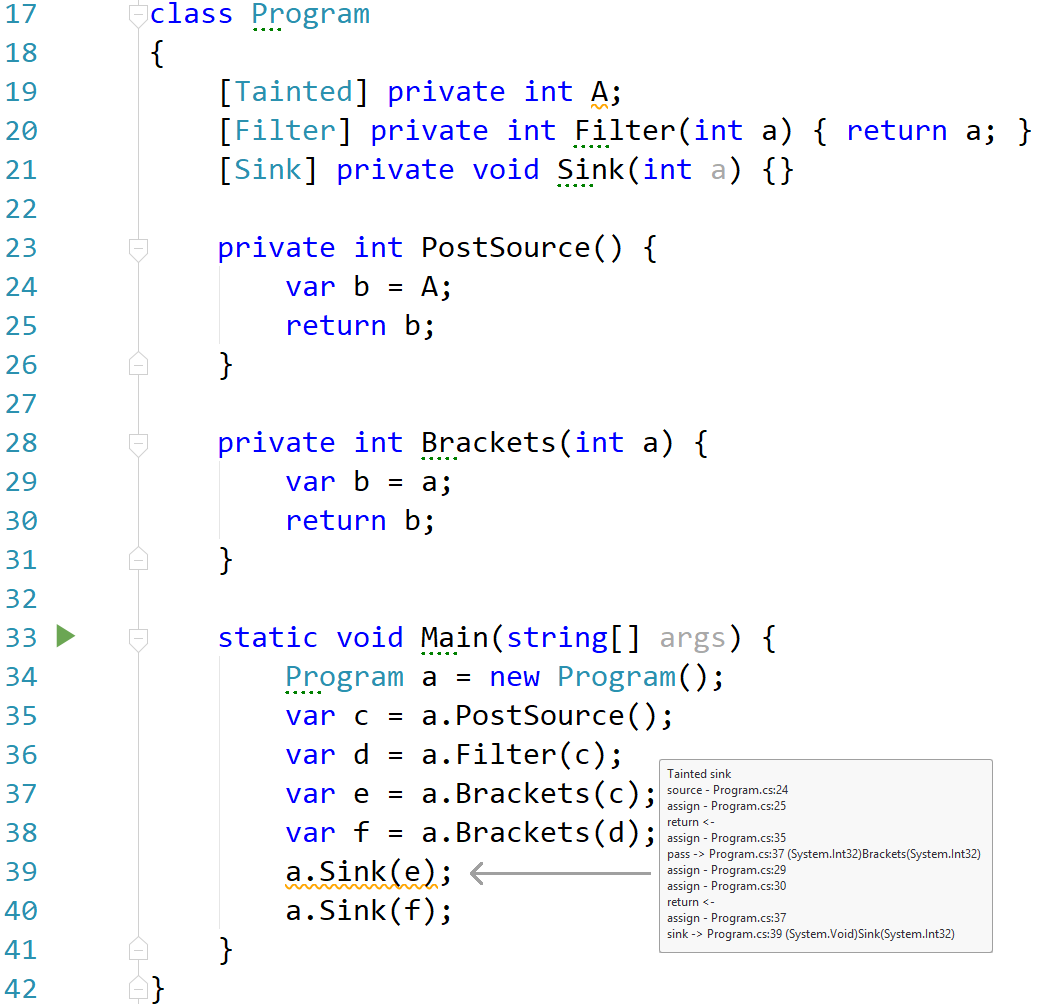
\includegraphics[width=\linewidth]{screenshots/ReturnsAndBrackets.png}
	\caption{Flow sensitivity}
	\label{fig:ReturnsAndBrackets}
\end{figure}

Secondly, the solution has the limited context sensitivity. I.e. it allows to track propagation of objects that are tainted by assigning of some fields inside them both by their own methods and by outer code interacting with their fields directly.
The first case is shown at fig~\ref{fig:ObjectTainting}.
There is the field \textit{B} at the line 18. 
This field can be used widely in the logic of the \textit{Container} class and by this the tainting of this field is considered as the tainting of the whole object.
However, while processing of the method \textit{Store} during the analysis it is hard to decide what the object need to be tainted because in the inner context of \textit{Store} it is just \textit{this} object.
I.e. we must consider the calling context to make such decision.
So, the solution provides this opportunity which is shown by lines 33-36 where the first invocation of \textit{Store} leads to the tainting of object \textit{d} and the second invocation does not taint object \textit{e}.

\begin{figure}[h]
	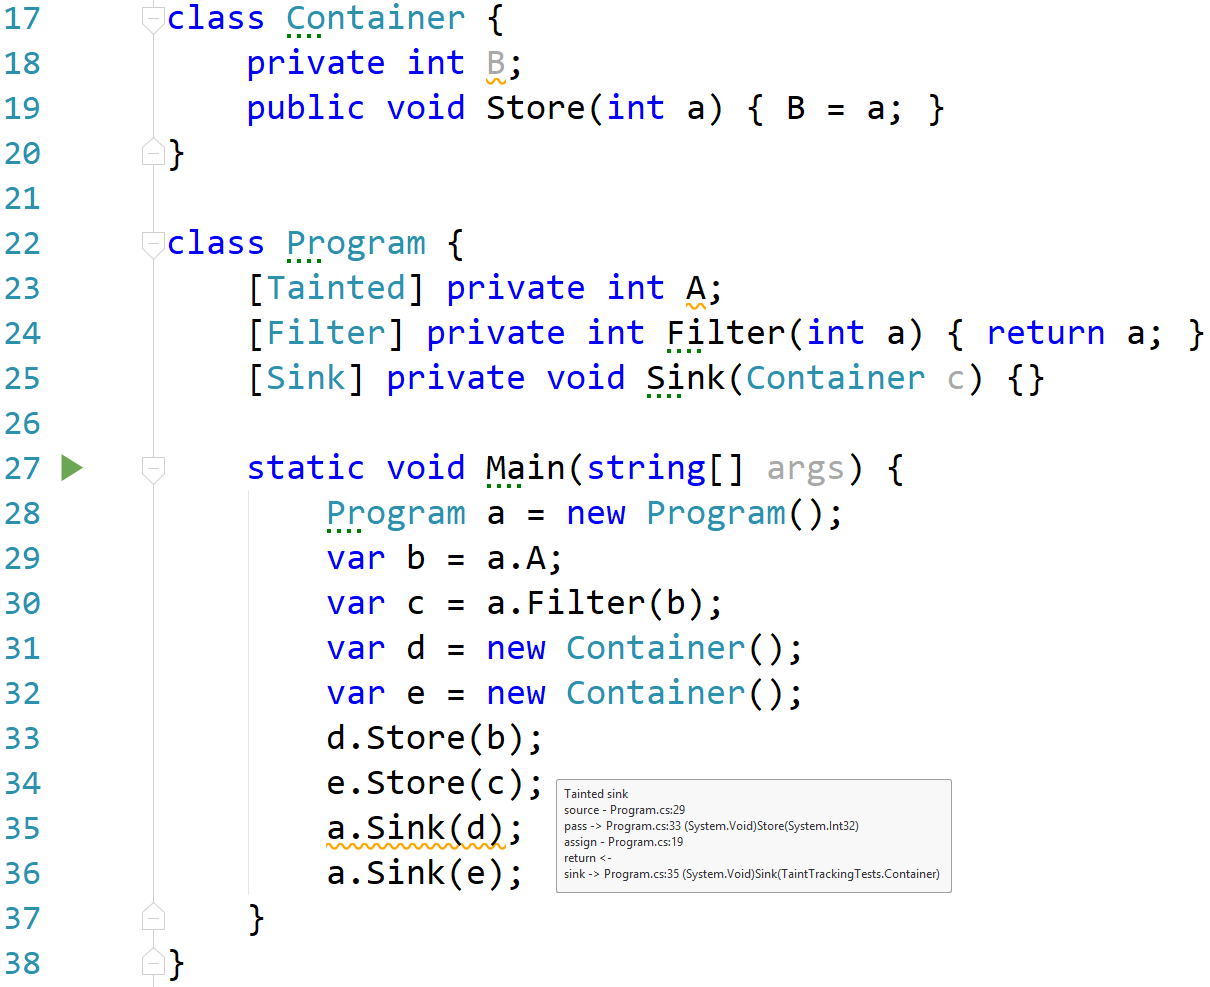
\includegraphics[width=\linewidth]{screenshots/ContextSensitivity.png}
	\caption{Tainting of an object by its own method}
	\label{fig:ObjectTainting}
\end{figure}

Finally, the solution works with any type of recursion and does not fall into infinite cycles.
It can be seen at fig.~\ref{fig:Recursion}.
This snippet contains two mutually recursive methods which pass the data to each other.
The solution checks all possible paths of passing even those which includes cyclic invocations and returns the passed variable to the point corresponding to the initial invocation.

\begin{figure}[h]
	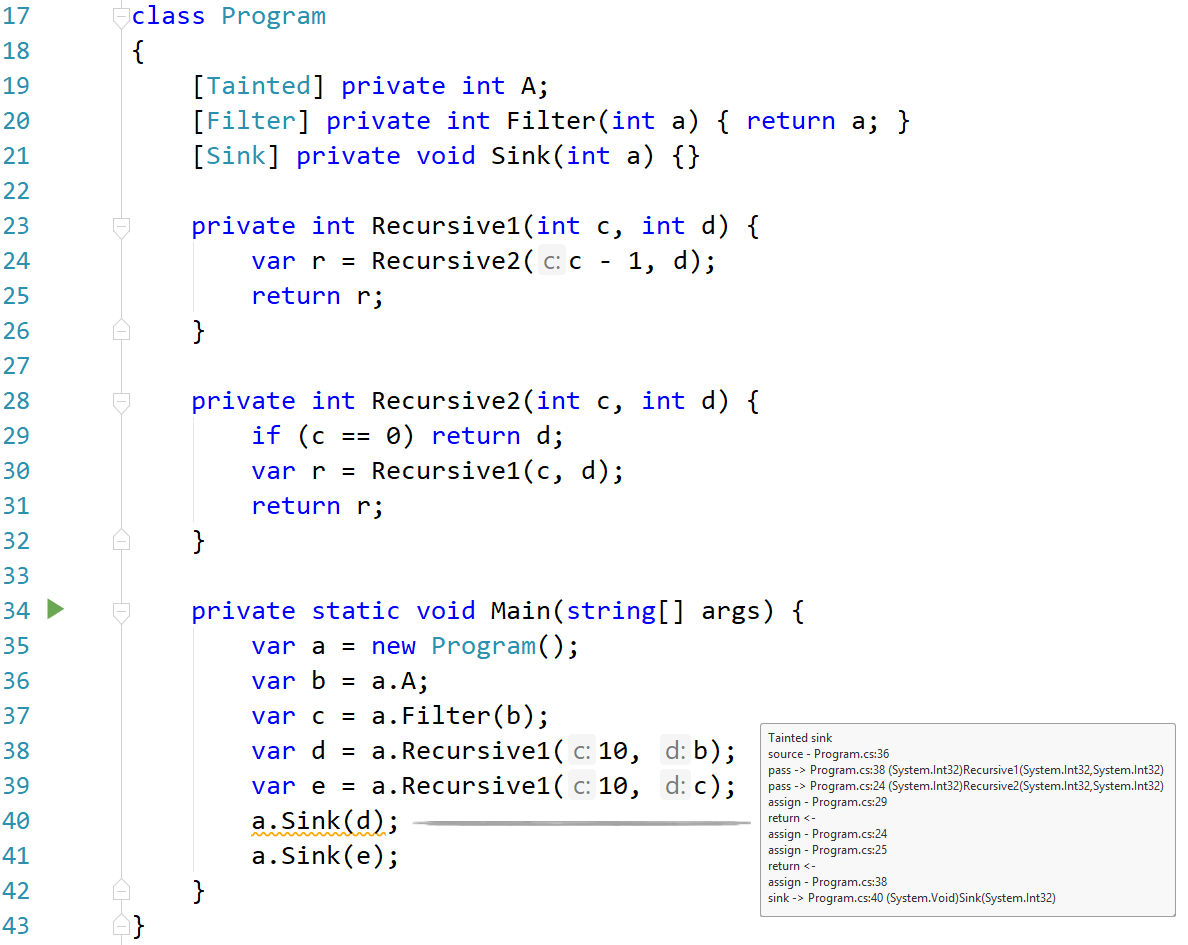
\includegraphics[width=\linewidth]{screenshots/Recursion.png}
	\caption{Recursive methods processing}
	\label{fig:Recursion}
\end{figure}

\subsection{Performance}

It is also necessary to measure the performance of the resulting solution.
Because the implemented taint tracking analysis forces to mark all participating entities manually, it is difficult to perform it on some large project.
However, there is another intermediate analysis which is runned before any other one to collect some information required by resolver.
In particular, it tracks propagation of all variables to discover all possible concrete types of each variable.
So, it involves each variable and each method in the whole program and thus the time and space required for execution of this analysis may be consistent estimation of the efficiency of the solution.

The code base that has been chosen as a source of data is the full solution of the Mono project.
(TODO: ADD SYSTEM CONFIGURATION).
The results is shown in the table~\ref{tab:Performance}.

\begin{table}[h]
	\begin{tabular}{|l|l|l|l|l|}
	\hline
		Project & Classes & Methods & \begin{tabular}[c]{@{}l@{}}Execution \\ time (s)\end{tabular} & \begin{tabular}[c]{@{}l@{}}Allocated \\ memory (GB)\end{tabular} \\ \hline
		Mono & 21013 & 192745 & $21\pm 0.5$ & $\sim 4.2$ \\ \hline
	\end{tabular}
	\caption{Performance}
	\label{tab:Performance}
\end{table}


\section{Conclusion}

We propose and implement in C\# programming language the generic framework for interprocedural static code analysis implementation.
This framework allows one to implement arbitrary interprocedural analysis in terms of CFL-reachability.
By using the proposed framework, we implement a plugin upon ReSharper infrastructure which provides simple taint analysis and demonstrate that our solution can handle important real-world cases.
Also we show that the proposed framework can be used for real-world solutions analysis.

One of the directions for future work is a creation of analysis and its evaluation on real-world projects.
By this way, we want to get information which helps to improve the usability of our framework: tune performance, improve API, etc.
Also we should improve documentation and create more examples of usage.

Another direction is a practical evaluation of automatic fix location prediction by using minimum cuts method~\cite{10.1007/978-3-319-63390-9_27}.

Also we want to compare the proposed approach with other generic CFL-reachability based approaches for interprocedural code analysis cretion. For example, fith generation-based approach~\cite{LPAR-21:Cauliflower_Solver_Generator_for}, which idea is similar to parser generators.


\bibliographystyle{ACM-Reference-Format}
\bibliography{IDE_Friendly_Interprocedural_Analyser}

\end{document}
